\documentclass{article}
\usepackage[utf8]{inputenc}
\usepackage{mathtools}
\usepackage{whilecode2}
\usepackage{listings}
\usepackage{fancyhdr}
\usepackage{graphicx}
\usepackage[colorlinks=true, allcolors=blue]{hyperref}
\pagestyle{fancy}
\lhead{Iván López Cervantes}
\rhead{\thepage}
\cfoot{}
\author{Ivan Lopez Cervantes }

\date{}
\begin{document}
\title{Práctica 3}
\maketitle


\maketitle

\section{Ejercicio 1}
Define la MT solución del ejercicio 3.4 de la lista de problemas y prueba su correcto comportamiento
\subsection*{Solución}
Matriz de la MT:
\begin{equation*}
\begin{bmatrix}
0 & * & l & 1\\
0 & | & | & 0\\
1 & * & | & 2\\
1 & | & l & 1\\
2 & * & l & 3\\
2 & | & r & 2\\
3 & * & l & 4\\
3 & | & * & 3\\
4 & * & h & 4\\
4 & | & * & 4\\
\end{bmatrix}
\end{equation*}
Máquina de Turing definida en JFLAP
\begin{figure}[h]
    \centering
    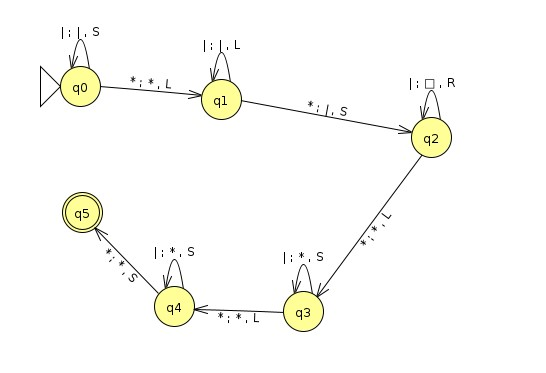
\includegraphics[scale=0.5]{MT.jpg}
\end{figure}
\newpage
\section{Ejercicio 2}
Define una función recursiva para la suma de tres valores.
\subsection*{Solución}
Función recursiva para la suma 3 valores: \\
$<<\pi^1_1 | \sigma(\pi^3_3)> | \sigma(\pi^4_4)>$\\
Ejemplo de ejecución:
\begin{figure}[h]
    \centering
    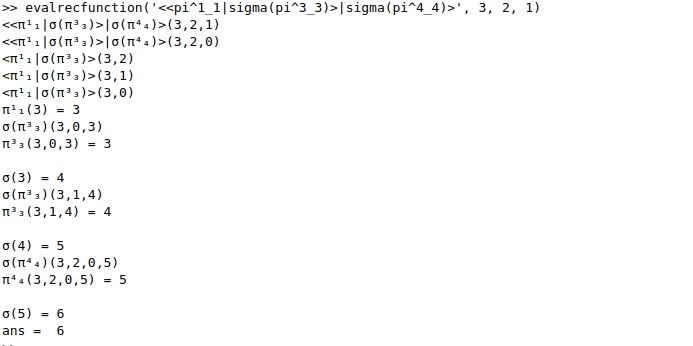
\includegraphics[scale=0.5]{Recursividad.jpg}
\end{figure}

\section{Ejercicio 3}
Implementa un programa WHILE que compute la suma de tres valores. Deberás usar una variable auxiliar que acumule el resultado de la suma.
\subsection*{Solución}
Programa WHILE que computa la suma de 3 valores:\\ 
\whileprogram{Q}{3}{
 
}{s}

\begin{whilecode}[H]

 \While{$X_2 \not = 0$}{
  $X_1 \Assig X_1 + 1$\;
  $X_2 \Assig X_2 - 1$\;
 }
 \While{$X_3 \not = 0$}{
  $X_1 \Assig X_1 + 1$\;
  $X_3 \Assig X_3 - 1$\;
 }
\end{whilecode}

\end{document}
